\chapter{Analysis Process and Result}

The Lyapunov function approach require 3 components which forms the optimzation problem described in chapter 3 to produce a worst-case performance convergence rate: the state update matrices, the constraints formed by the interpolation conditions and the performance measure. These components are derived from the input provided to JuPE which undergo transformations before they can be used to create an optimization problem in the JuMP modelling language, the process of which can be described in 3 steps:
\begin{enumerate}
    \item JuPE automatically uses the input provided to form a systematic charaterization the analysis problem using data structures described in chapter 4, including how the algorithm being analyzed updates, the constraints created by the interpolation conditions of the class of function and the performance measure.
    \item These data structures are converted to real number vectors and matrices that represent the updated state of the algorithm and each algorithm in the form of the a linear function of the initial states and inputs.
    \item An optimization problem is created inside a JuMP model using these representations and solved to verify whether a certain convergence rate is feasible for a given problem. This process is repeated with different convergence rates as JuPE search for the lowest feasible convergence rate.
\end{enumerate}

This chapter details the analysis process, including how these steps are performed for component and how the optmization problem is formed and solved to derive worst-case performancce convergence rate. In addition, the analysis result of three algorithms over smooth strongly convex functions will also be detailed as an example of the result produced by algorithm analysis.

\subsection*{Real scalars and linear form}

In JuPE, when a variable expression is defined in an inner product space, which include states of an algorithm, the starting and goal points and the gradient of a function at a point, it is a vector. However, all three components needed to form the Lyapunov functions exist as real scalars. Constraints created by the interpolation conditions are applied to the inner product and norm of state and input vectors, which are real scalar as can be seen in \ref{ex_orc_constraints}, while the performance measure formed from state vectors has to be real scalars in order to be measured. Similarly, the state update matrix used to construct the Lyapunov function is formed as the inner product of state space matrices representing the algorithm and therefore are scalars.

As the JuMP modeling language does not support the expression and constraint data structures presented in chapter 4, how the components of the Lyapunov function are represented must be transformed to real numbers before they can be inputted into a JuMP model. And as all three components are created from real scalars formed from the states and inputs, JuPE achieve this by expressing these components as a linear function of real variable expressions. This process is done in three steps, which are:
\begin{enumerate}
    \item Of every expressions that has been created during the input process, define the initial state vector x as every real expressions which contain another expression in its next field.
\begin{figure}[h!]
    \begin{lstlisting}[mathescape]
x  = collect(v for v $\in $ vars if !ismissing(next(v)) && v isa R)
4-element Vector{R}:
    |x0|$^2$
    |xs|$^2$
    <x0,xs>
    <xs,x0>
\end{lstlisting}
\caption{Initial state real scalar expressions from example \ref{ex_analysis}}
\label{ex_initstate}
\end{figure}

    \item Defining an update state vector x$^+$ consisting of the next expression of every expression in the initial state. The input vector u is then defined as every real expression that exist in the decomposition of the updated state expressions but not in the initial state expressions.
    \begin{figure}[h!]
        \begin{lstlisting}[mathescape]    
x$^+$ = next(x)
4-element Vector{R}:
    <x0,xs> - 0.18181818181818182 <$\nabla $f(x0),xs>
    -0.18181818181818182 <$\nabla $f(x0),x0> + 0.03305785123966942 |$\nabla $f(x0)|$^2$ - 0.18181818181818182 <x0,$\nabla $f(x0)> + |x0|$^2$
    -0.18181818181818182 <xs,$\nabla $f(x0)> + <xs,x0>
    |xs|$^2$

u  = collect(setdiff(variables(x$^+$), variables(x)))
5-element Vector{Expression}:
    <xs,$\nabla $f(x0)>
    <x0,$\nabla $f(x0)>
    <$\nabla $f(x0),xs>
    <$\nabla $f(x0),x0>
    |$\nabla $f(x0)|$^2$
        \end{lstlisting}    
    \caption{Updated state and input real scalar expressions from example \ref{ex_analysis}}
    \label{ex_updatedstate_input}
    \end{figure}
    \item The initial state and input vector [x; u] can now form every expression in the optimization problem, which means any real scalar expression can be transformed into a linear function of [x; u] by finding the matrix or vector with which to multiply [x; u] to find that expression. This matrix, which will be refered to as the linear form of an expression, can be derived by finding the values of each expression in the initial and state input vector present in the expression's decomposition dictionary.
\end{enumerate}

\begin{figure}[h!]
    \begin{lstlisting}[mathescape] 
linear_form = vec(linearform([x; u] => x0^2 - 3*(x0'*xs)))
linear_form'*[x; u]
Scalar in R
  Decomposition: -3 <xs,x0> + |x0|$^2$
\end{lstlisting}    
\caption{Example of linear form of a scalar expression \ref{ex_analysis}}
\label{ex_linearform}
\end{figure}

\section{Performance measure}
As the performance measure is defined, a scalar expression is created. The linear form matrix of the performance measure is the first of the three components needed to form the Lyapunov function. For example, the performance measure in \ref{ex_analysis}, which is defined as $(x0-xs)^2$ and which evaluates into $|x0|^2 - <xs, x0> - <x0, xs> + |xs|^2$, is:
\begin{figure}[h!]
\begin{lstlisting}[mathescape]
$\mathcal{P} $ = vec(linearform( [x; u] => performance ))
9-element Vector{Int64}:
    -1
    1
    -1
    1
    0
    0
    0
    0
    0
\end{lstlisting}
\caption{Linear form matrix of expression $(x0-xs)^2$}
\label{ex_linearform}
\end{figure}

\section{Algorithm and state update}
% \subsection*{State space matrix and their linear form formulation}
\ref{ex_analysis} shows the algorithm to be analyzed is inputted into JuPE first by defining an initial state and how a 'next' state is updated from the initial state. The initial state is defined to be a vector in an inner product space, and the updated state is a linear function of one or multiple initial state and the gradient of the function evaluated at some point. While the gradient descent algorithm updates using only one state and evaluate the gradient at the previous state, if an algorithm updates using multiple past states or the gradient at an interpolated point, these vectors will also have to be defined.

The forming of the algorithm can then be completed by defining the relationship between states and their next states using the "=>" operation, which updates the next field of every expression in the decomposition of which there is the state on the left hand side of the operation.

\begin{figure}[h!]
	\begin{lstlisting}[mathescape]
next(x0)

Vector in R$^n$
  Label: x1
  Decomposition: -0.18181818181818182 $\nabla $f(x0) + x0
  Associations: Dual => x1*

next(x0'*xs)

  Scalar in R
    Decomposition: -0.18181818181818182 <xs,$ \nabla $f(x0)> + <xs,x0>
\end{lstlisting}
\caption{next field of a state vector expressions and a scalar formed from a state expression}
\label{ex_next}
\end{figure}

The initial and update state vectors are created in \ref{ex_initstate} and \ref{ex_updatedstate_input}, their linear form matrices is the second of the three components needed to formulate the Lyapunov function and can be formed as:

\begin{figure}[h!]
    \begin{lstlisting}[mathescape]
X  = linearform([x; u] => x)
    4x9 Matrix{Int64}:
    1  0  0  0  0  0  0  0  0
    0  1  0  0  0  0  0  0  0
    0  0  1  0  0  0  0  0  0
    0  0  0  1  0  0  0  0  0

X$^+$ = linearform([x; u] => x$^+$)
    4x9 Matrix{Real}:
    1  0  0  0   0          0         -0.181818  0           0
    0  1  0  0  -0.181818   0          0         0.0330579  -0.181818
    0  0  1  0   0         -0.181818   0         0           0
    0  0  0  1   0          0          0         0           0
    
    \end{lstlisting}
    \caption{Linear form state matrices x and x$^+$}
    \label{ex_linearform_state}
    \end{figure}

% \subsection*{State space in Lyapunov function}
Following the steps presented in chapter 3, the Lyapunov function can begin to be formed thusly:
\begin{description}
    \item [Optimization variable P] An optimization variable P is defined in the JuMP model as a JuMP variable. Once JuMP and the solver start optimizing the problem, P is one of the variable that will be optimized to produce a solution
    \item [Lyapunov function for ] The first Lyapunov function L1 is formed as: L1 = $\mathcal{P} $ - X'*P.
    \item [Lyapunov function for decreasing] The second Lyapunov function L2 is formed as: L2 = X$^+ $'*P - $\rho $*X'*P.    
\end{description}

\section{Constraints}
As presented in 4.3, the oracle created from the class of function provided as the input automatically create the constraints that interpolate that class of function. These constraints are linearized and added to the optimization in 2 steps:
\begin{description}
    \item [Optimization variable multipliers] For each constraint, two optimization variables are defined similar to optimization variable P. If the constraint is created from the interpolation condition for the transpose of state vectors and is applied to a matrix of real scalar expressions, the optimization variable will be a matrix sharing the same size with the matrix constrained. If the constraint is created from the interpolation conditions of the class of function and is applied to a single real scalar expression, the optimization problem created will have a size of 1. Depending on the type of constraint.
    \item [Constraint on multiplier] The JuMP variables multipliers are constrained in the JuMP model depending on the constraint expression they were created from: The multiplier is not constrained if the expression is constrained to be zero, is constrained to be non-negative if the expression is constrained to be non-negative, and is constrained to be symmetrical and in the JuMP supported positive semidefinite cone if the expression is constrained to be positive semidefinite.
    \item [Linear form of constraints] The linear form of each constraint scaled by the multiplier can then be created and added to the Lyapunov functions.
\end{description}

If the expression constrained is a single real scalar, the linear form of the constraint is derived similarly to the linear form of the performance measure or state space matrices but scaled by the multiplier. Suppose we have the constraint $(x0 - xs)^2 \geq 0$ and matrix $\bmat{x\\ u} = \bmat{|x0|^2\\ <xs, x0>\\ |xs|^2}$, the linear form of the constraint in terms of $\bmat{x\\ u}$, denoted as $M$ would be:

\begin{subequations} \label{eqn:constraint_single}
	\begin{align}
    \lambda * (x0 - xs)^2 &= M * \bmat{|x0|^2\\ <xs, x0>\\ |xs|^2} \label{eq_cons_single1}       \\
	M &= \bmat{\lambda& 2\lambda & \lambda} \label{eq_cons_single2}
	\end{align}
\end{subequations}

If the expression constrained and its corresponding multiplier is a vector of expression, the linear form of the constraint is derived as the linear form of the inner product between the multiplier vector and the constraint expression vector. Suppose we have a constraint vector $\bmat{(x0-xs)^2 \\ (x0-xs)^2-3*|xs|^2} \geq 0$ and the same $\bmat{x\\ u}$ matrix as \ref{eqn:constraint_single}, the linear form of the constraint in terms of $\bmat{x\\ u}$, denoted as $M$ would be:

\begin{subequations} \label{eqn:constraint_vector}
	\begin{align}
    \bmat{\lambda _1 & \lambda _2} * \bmat{(x0 - xs)^2 \\ (x0 - xs)^2-3*|xs|^2} &= M * \bmat{|x0|^2\\ <xs, x0>\\ |xs|^2} \label{eq_cons_vector1}       \\
	M &= \bmat{\lambda & -\lambda & \lambda \\ \lambda & -\lambda & -2*\lambda} \label{eq_cons_vector2}
	\end{align}
\end{subequations}

In all three cases, the resulting linear form matrix is the linear form of the constraint expression scaled by the JuMP variable multipliers. As 2 multiplier variables are defined for each constraints, the resulting linear form matrices are each transformed into a vector and added the two Lyapunov functions.

\section{Derived feasibility and bisection search}

\section{Result}
After running JuPE to perform algorithm analysis on three algorithms (GD), (HB), and (FG) on classes of m strong L smooth convex function where the condition number L/m are chosen between 1 and 10, we get 
\begin{figure}[h]
    \centering
    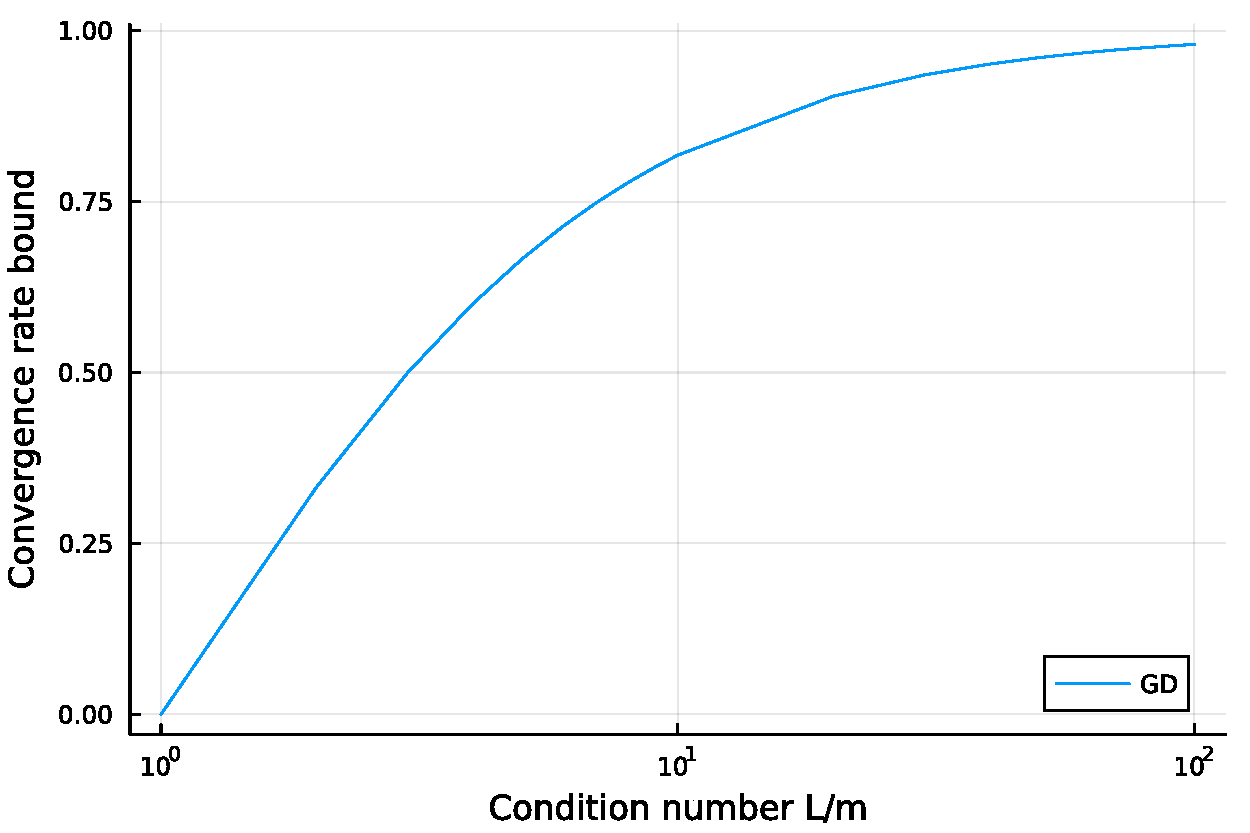
\includegraphics[width = .8 \textwidth]{plot.pdf}
    \caption{Convergence rate}
    \label{plot_result}
\end{figure}